\documentclass[12pt,titlepage]{article}
\usepackage[margin=1in]{geometry}
\usepackage{fancyhdr}
\usepackage{amsmath}
\usepackage{graphicx}
\usepackage{tikz}
\setlength\parindent{0pt}
\fancyhf{}
\rfoot{Page \thepage}

\begin{document}
\begin{titlepage}
	\centering
	\vfill
	{\bfseries\Large
		Joseph Morgan\\
		\large
		Homework 13\\
		\vskip2cm
		CISP440\\
	}
	\vfill
	\vfill
	\vfill
\end{titlepage}
\section*{\textit{Section 10.1}}
\subsection*{\textit{Draw the transition diagram of the finite state machine $(I, O, S, f, g, o_0)$}}
\subsubsection*{2. $I = \{a, b\}, O = \{0, 1\}, S = \{o_0, o_1\}$}
\begin{center}
	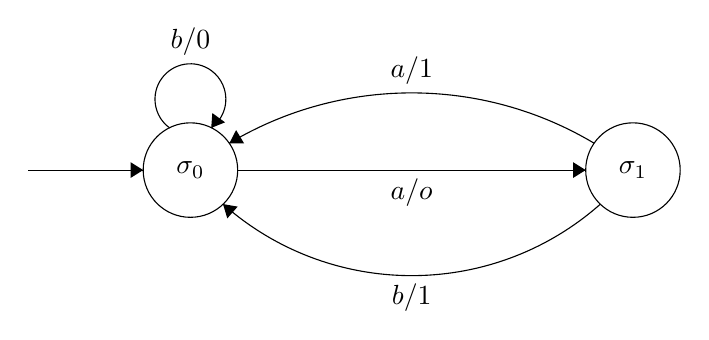
\begin{tikzpicture}[scale=0.2]
		\tikzstyle{every node}+=[inner sep=0pt]
		\draw [black] (25.4,-27.4) circle (3);
		\draw (25.4,-27.4) node {$\sigma_0$};
		\draw [black] (53.5,-27.4) circle (3);
		\draw (53.5,-27.4) node {$\sigma_1$};
		\draw [black] (24.077,-24.72) arc (234:-54:2.25);
		\draw (25.4,-20.15) node [above] {$b/0$};
		\fill [black] (26.72,-24.72) -- (27.6,-24.37) -- (26.79,-23.78);
		\draw [black] (28.4,-27.4) -- (50.5,-27.4);
		\fill [black] (50.5,-27.4) -- (49.7,-26.9) -- (49.7,-27.9);
		\draw (39.45,-27.9) node [below] {$a/o$};
		\draw [black] (51.428,-29.565) arc (-48.49676:-131.50324:18.076);
		\fill [black] (27.47,-29.56) -- (27.74,-30.47) -- (28.4,-29.72);
		\draw (39.45,-34.6) node [below] {$b/1$};
		\draw [black] (27.866,-25.695) arc (120.85331:59.14669:22.588);
		\fill [black] (27.87,-25.7) -- (28.81,-25.71) -- (28.3,-24.86);
		\draw (39.45,-22) node [above] {$a/1$};
		\draw [black] (15.1,-27.4) -- (22.4,-27.4);
		\fill [black] (22.4,-27.4) -- (21.6,-26.9) -- (21.6,-27.9);
	\end{tikzpicture}
\end{center}
\subsubsection*{5. $I = \{a, b, c\}, O = \{0, 1, 2\}, S = \{o_0, o_1, o_2, o_3\}$}
\begin{center}
	\begin{tikzpicture}[scale=0.2]
		\tikzstyle{every node}+=[inner sep=0pt]
		\draw [black] (10.7,-31.1) circle (3);
		\draw (10.7,-31.1) node {$\sigma_0$};
		\draw [black] (28.5,-31.1) circle (3);
		\draw (28.5,-31.1) node {$\sigma_1$};
		\draw [black] (50.8,-31.1) circle (3);
		\draw (50.8,-31.1) node {$\sigma_2$};
		\draw [black] (69.6,-31.1) circle (3);
		\draw (69.6,-31.1) node {$\sigma_3$};
		\draw [black] (13.583,-30.275) arc (102.80312:77.19688:27.153);
		\fill [black] (25.62,-30.28) -- (24.95,-29.61) -- (24.73,-30.59);
		\draw (19.6,-29.1) node [above] {$a/1$};
		\draw [black] (9.377,-28.42) arc (234:-54:2.25);
		\draw (10.7,-23.85) node [above] {$b/1$};
		\fill [black] (12.02,-28.42) -- (12.9,-28.07) -- (12.09,-27.48);
		\draw [black] (48.384,-32.876) arc (-56.37415:-123.62585:31.843);
		\fill [black] (48.38,-32.88) -- (47.44,-32.9) -- (47.99,-33.74);
		\draw (30.75,-38.7) node [below] {$c/2$};
		\draw [black] (25.633,-31.978) arc (-76.34199:-103.65801:25.55);
		\fill [black] (13.57,-31.98) -- (14.23,-32.65) -- (14.46,-31.68);
		\draw (19.6,-33.2) node [below] {$a/2$};
		\draw [black] (31.5,-31.1) -- (47.8,-31.1);
		\fill [black] (47.8,-31.1) -- (47,-30.6) -- (47,-31.6);
		\draw (39.65,-31.6) node [below] {$b/0\mbox{ }&\mbox{ }c/0$};
		\draw [black] (66.771,-32.094) arc (-74.205:-105.795:24.142);
		\fill [black] (66.77,-32.09) -- (65.87,-31.83) -- (66.14,-32.79);
		\draw (60.2,-33.51) node [below] {$a/1$};
		\draw [black] (53.629,-30.109) arc (105.7539:74.2461:24.2);
		\fill [black] (66.77,-30.11) -- (66.14,-29.41) -- (65.86,-30.37);
		\draw (60.2,-28.7) node [above] {$b/0$};
		\draw [black] (13.187,-29.424) arc (121.41785:58.58215:33.692);
		\fill [black] (13.19,-29.42) -- (14.13,-29.43) -- (13.61,-28.58);
		\draw (30.75,-23.98) node [above] {$c/1$};
		\draw [black] (67.134,-32.806) arc (-57.85412:-122.14588:33.987);
		\fill [black] (30.97,-32.81) -- (31.38,-33.66) -- (31.91,-32.81);
		\draw (49.05,-38.52) node [below] {$a/2$};
		\draw [black] (30.99,-29.428) arc (121.39482:58.60518:34.669);
		\fill [black] (30.99,-29.43) -- (31.93,-29.44) -- (31.41,-28.58);
		\draw (49.05,-23.85) node [above] {$b/0$};
		\draw [black] (67.555,-33.294) arc (-45.2065:-134.7935:38.896);
		\fill [black] (12.75,-33.29) -- (12.96,-34.21) -- (13.67,-33.5);
		\draw (40.15,-45.09) node [below] {$c/2$};
		\draw [black] (3.8,-31.1) -- (7.7,-31.1);
		\fill [black] (7.7,-31.1) -- (6.9,-30.6) -- (6.9,-31.6);
	\end{tikzpicture}
\end{center}
\subsection*{\textit{In Exercises 6-10, find the sets I, O, and S, the initial state, and the table
defining the next state and output functions for each finite-state machine}}
\subsubsection*{7.}
\begin{center}
	\begin{tabular}{|c|c c|c c|}
		\hline
		\bf{\textit{S}}& \bf{\textit{f}} & & \bf{\textit{g}} & \\ \hline
															& a  & b & a & b \\ \hline
		$A & A & B & 0 & 1$ \\
		$B & A & C & 0 & 1$ \\
		$C & C & A & 1 & 0$ \\ \hline
	\end{tabular}
\end{center}
\subsubsection*{10.}
\begin{center}
	\begin{tabular}{|c|c c c|c c c|}
		\hline
		\bf{\textit{S}}& \bf{\textit{f}} & & & \bf{\textit{g}} & & \\ \hline
																 & a  & b & c & a & b & c\\ \hline
		$B & A & D & D & 2 & 0 & 0 $ \\
		$A & B & A & C & 1 & 0 & 2 $ \\
		$C & A & C & D & 0 & 1 & 2 $ \\
		$D & D & C & A & 2 & 2 & 0 $ \\ \hline
	\end{tabular}
\end{center}
\subsection*{\textit{In Exercises 11-20, find the output string for the given input string
and finite-state machine.}}
\subsubsection*{12. \textit{abba}; Exercise 1}
Output is: 0111
\subsubsection*{16. \textit{aaa}; Exercise 6}
Output is: 011
\subsubsection*{17. \textit{aabbabaab}; Exercise 7}
Output is: 001110001
\subsubsection*{19. \textit{bbababbabaaa}; Exercise 9}
Output is: 010000000001
\subsection*{\textit{In Exercises 21-26, design a finite-state machine having the given properties.
The input is always a bit string.}}
\subsubsection*{22. Outputs 1 if \textit{k} 1's have been input, where \textit{k} is a multiple of 3;
otherwise, output 0.}
\begin{center}
	\begin{tabular}{|c|c c|c c|}
		\hline
		\bf{\textit{S}}& \bf{\textit{f}} & & \bf{\textit{g}} & \\ \hline
															& 0  & 1 & 0 & 1 \\ \hline
		$s_0 & s_0 & s_1 & 0 & 0$ \\
		$s_1 & s_0 & s_2 & 0 & 0$ \\
		$s_2 & s_0 & s_0 & 0 & 1$ \\ \hline
	\end{tabular}
\end{center}
\begin{center}
	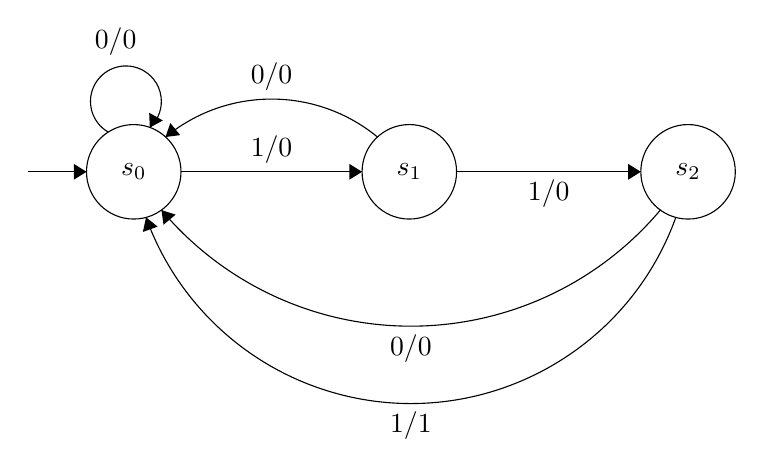
\begin{tikzpicture}[scale=0.2]
		\tikzstyle{every node}+=[inner sep=0pt]
		\draw [black] (26.5,-29.3) circle (3);
		\draw (26.5,-29.3) node {$s_0$};
		\draw [black] (44,-29.3) circle (3);
		\draw (44,-29.3) node {$s_1$};
		\draw [black] (61.7,-29.3) circle (3);
		\draw (61.7,-29.3) node {$s_2$};
		\draw [black] (29.5,-29.3) -- (41,-29.3);
		\fill [black] (41,-29.3) -- (40.2,-28.8) -- (40.2,-29.8);
		\draw (35.25,-28.8) node [above] {$1/0$};
		\draw [black] (47,-29.3) -- (58.7,-29.3);
		\fill [black] (58.7,-29.3) -- (57.9,-28.8) -- (57.9,-29.8);
		\draw (52.85,-29.8) node [below] {$1/0$};
		\draw [black] (60.923,-32.194) arc (-19.82529:-160.17471:17.883);
		\fill [black] (27.28,-32.19) -- (27.08,-33.12) -- (28.02,-32.78);
		\draw (44.1,-44.51) node [below] {$1/1$};
		\draw [black] (59.942,-31.727) arc (-40.07255:-139.92745:20.702);
		\fill [black] (28.26,-31.73) -- (28.39,-32.66) -- (29.16,-32.02);
		\draw (44.1,-39.6) node [below] {$0/0$};
		\draw [black] (24.89,-26.783) arc (240.34019:-47.65981:2.25);
		\draw (25.35,-21.94) node [above] {$0/0$};
		\fill [black] (27.52,-26.49) -- (28.35,-26.04) -- (27.48,-25.55);
		\draw [black] (28.518,-27.094) arc (129.44581:50.55419:10.596);
		\fill [black] (28.52,-27.09) -- (29.45,-26.97) -- (28.82,-26.2);
		\draw (35.25,-24.18) node [above] {$0/0$};
		\draw [black] (19.8,-29.3) -- (23.5,-29.3);
		\fill [black] (23.5,-29.3) -- (22.7,-28.8) -- (22.7,-29.8);
	\end{tikzpicture}
\end{center}
\subsubsection*{25. Outputs 1 when it sees 101 and thereafter; otherwise, outputs 0.}
\begin{center}
	\begin{tabular}{|c|c c|c c|}
		\hline
		\bf{\textit{S}}& \bf{\textit{f}} & & \bf{\textit{g}} & \\ \hline
										 & 0  & 1 & 0 & 1 \\ \hline
		$s_0 & s_0 & s_1 & 0 & 0$ \\
		$s_1 & s_2 & s_1 & 0 & 0$ \\
		$s_2 & s_0 & s_3 & 0 & 1$ \\
		$s_3 & s_3 & s_3 & 1 & 1$ \\ \hline
	\end{tabular}
\end{center}
\begin{center}
	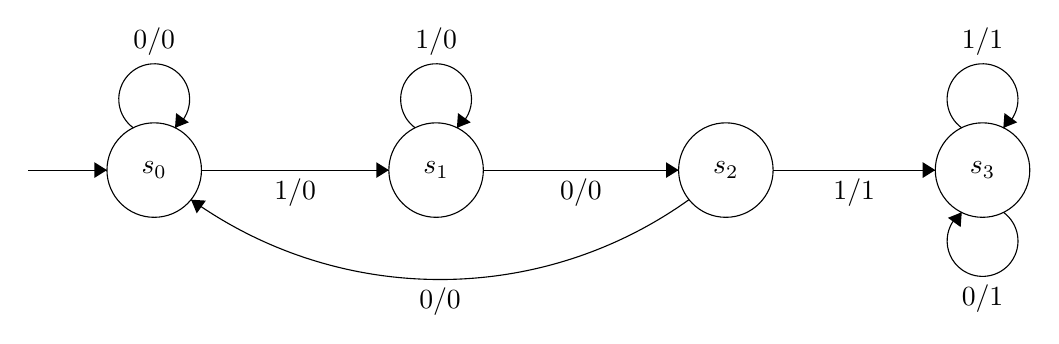
\begin{tikzpicture}[scale=0.2]
		\tikzstyle{every node}+=[inner sep=0pt]
		\draw [black] (12,-29.5) circle (3);
		\draw (12,-29.5) node {$s_0$};
		\draw [black] (29.9,-29.5) circle (3);
		\draw (29.9,-29.5) node {$s_1$};
		\draw [black] (48.3,-29.5) circle (3);
		\draw (48.3,-29.5) node {$s_2$};
		\draw [black] (64.6,-29.5) circle (3);
		\draw (64.6,-29.5) node {$s_3$};
		\draw [black] (10.677,-26.82) arc (234:-54:2.25);
		\draw (12,-22.25) node [above] {$0/0$};
		\fill [black] (13.32,-26.82) -- (14.2,-26.47) -- (13.39,-25.88);
		\draw [black] (28.577,-26.82) arc (234:-54:2.25);
		\draw (29.9,-22.25) node [above] {$1/0$};
		\fill [black] (31.22,-26.82) -- (32.1,-26.47) -- (31.29,-25.88);
		\draw [black] (45.961,-31.377) arc (-54.4203:-125.5797:27.175);
		\fill [black] (14.34,-31.38) -- (14.7,-32.25) -- (15.28,-31.44);
		\draw (30.15,-36.95) node [below] {$0/0$};
		\draw [black] (51.3,-29.5) -- (61.6,-29.5);
		\fill [black] (61.6,-29.5) -- (60.8,-29) -- (60.8,-30);
		\draw (56.45,-30) node [below] {$1/1$};
		\draw [black] (15,-29.5) -- (26.9,-29.5);
		\fill [black] (26.9,-29.5) -- (26.1,-29) -- (26.1,-30);
		\draw (20.95,-30) node [below] {$1/0$};
		\draw [black] (32.9,-29.5) -- (45.3,-29.5);
		\fill [black] (45.3,-29.5) -- (44.5,-29) -- (44.5,-30);
		\draw (39.1,-30) node [below] {$0/0$};
		\draw [black] (63.277,-26.82) arc (234:-54:2.25);
		\draw (64.6,-22.25) node [above] {$1/1$};
		\fill [black] (65.92,-26.82) -- (66.8,-26.47) -- (65.99,-25.88);
		\draw [black] (65.923,-32.18) arc (54:-234:2.25);
		\draw (64.6,-36.75) node [below] {$0/1$};
		\fill [black] (63.28,-32.18) -- (62.4,-32.53) -- (63.21,-33.12);
		\draw [black] (4,-29.5) -- (9,-29.5);
		\fill [black] (9,-29.5) -- (8.2,-29) -- (8.2,-30);
	\end{tikzpicture}
\end{center}

\section*{\textit{Section 10.2}}
\subsection*{\textit{In Exercises 1-3, show that each finite-state machine is a
finite-state automaton and redraw the transition diagram as the diagram of a finate-state automaton.}}
\subsubsection*{2.}
\begin{center}
	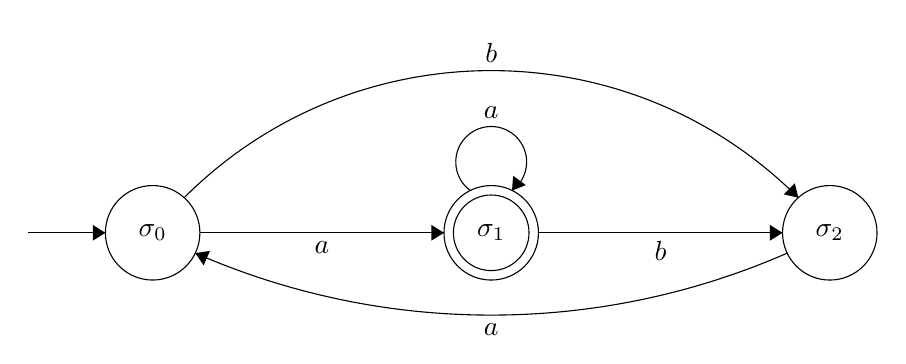
\begin{tikzpicture}[scale=0.2]
		\tikzstyle{every node}+=[inner sep=0pt]
		\draw [black] (19.5,-30.5) circle (3);
		\draw (19.5,-30.5) node {$\sigma_0$};
		\draw [black] (41,-30.5) circle (3);
		\draw (41,-30.5) node {$\sigma_1$};
		\draw [black] (41,-30.5) circle (2.4);
		\draw [black] (62.5,-30.5) circle (3);
		\draw (62.5,-30.5) node {$\sigma_2$};
		\draw [black] (11.6,-30.5) -- (16.5,-30.5);
		\fill [black] (16.5,-30.5) -- (15.7,-30) -- (15.7,-31);
		\draw [black] (21.503,-28.269) arc (134.97158:45.02842:27.587);
		\fill [black] (60.5,-28.27) -- (60.28,-27.35) -- (59.58,-28.06);
		\draw (41,-19.7) node [above] {$b$};
		\draw [black] (59.793,-31.791) arc (-66.34394:-113.65606:46.835);
		\fill [black] (22.21,-31.79) -- (22.74,-32.57) -- (23.14,-31.65);
		\draw (41,-36.23) node [below] {$a$};
		\draw [black] (39.677,-27.82) arc (234:-54:2.25);
		\draw (41,-23.25) node [above] {$a$};
		\fill [black] (42.32,-27.82) -- (43.2,-27.47) -- (42.39,-26.88);
		\draw [black] (22.5,-30.5) -- (38,-30.5);
		\fill [black] (38,-30.5) -- (37.2,-30) -- (37.2,-31);
		\draw (30.25,-31) node [below] {$a$};
		\draw [black] (44,-30.5) -- (59.5,-30.5);
		\fill [black] (59.5,-30.5) -- (58.7,-30) -- (58.7,-31);
		\draw (51.75,-31) node [below] {$b$};
	\end{tikzpicture}
\end{center}
\subsection*{\textit{In Exercises 13-17, determine whether the givin string is
accpeted by the given finite-state automaton.}}
\subsubsection*{15. aabaabb; Figure 10.2.5}
Yes, it would be accepted because the final state of the automaton is $\sigma_2$,
which is an accepted state.
\subsection*{\textit{In Exercises 21-31, draw the transition diagram of a
finite-state automaton that accepts the given set of strings over \{a, b\}}}
\subsubsection*{26. Contains \textit{m} \textit{a}'s where \textit{m} is a multiple of 3.}
$\sigma_0 = $ Nothing in input buffer.\\
$\sigma_2 = $ Number of \textit{m}'s in input buffer modulus 3 equals 1.\\
$\sigma_3 = $ Number of \textit{m}'s in input buffer modulus 3 equals 2.\\
$\sigma_4 = $ Number of \textit{m}'s in input buffer modulus 3 equals 0.\\
\begin{center}
	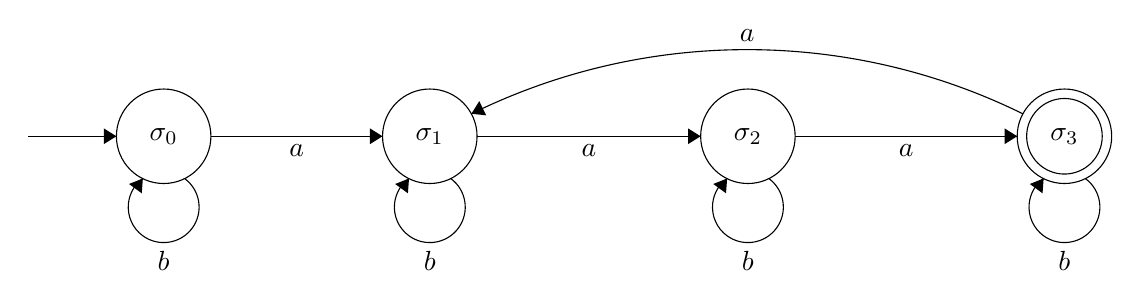
\begin{tikzpicture}[scale=0.2]
		\tikzstyle{every node}+=[inner sep=0pt]
		\draw [black] (13.5,-28.3) circle (3);
		\draw (13.5,-28.3) node {$\sigma_0$};
		\draw [black] (30.4,-28.3) circle (3);
		\draw (30.4,-28.3) node {$\sigma_1$};
		\draw [black] (50.6,-28.3) circle (3);
		\draw (50.6,-28.3) node {$\sigma_2$};
		\draw [black] (70.7,-28.3) circle (3);
		\draw (70.7,-28.3) node {$\sigma_3$};
		\draw [black] (70.7,-28.3) circle (2.4);
		\draw [black] (4.9,-28.3) -- (10.5,-28.3);
		\fill [black] (10.5,-28.3) -- (9.7,-27.8) -- (9.7,-28.8);
		\draw [black] (14.823,-30.98) arc (54:-234:2.25);
		\draw (13.5,-35.55) node [below] {$b$};
		\fill [black] (12.18,-30.98) -- (11.3,-31.33) -- (12.11,-31.92);
		\draw [black] (16.5,-28.3) -- (27.4,-28.3);
		\fill [black] (27.4,-28.3) -- (26.6,-27.8) -- (26.6,-28.8);
		\draw (21.95,-28.8) node [below] {$a$};
		\draw [black] (33.4,-28.3) -- (47.6,-28.3);
		\fill [black] (47.6,-28.3) -- (46.8,-27.8) -- (46.8,-28.8);
		\draw (40.5,-28.8) node [below] {$a$};
		\draw [black] (53.6,-28.3) -- (67.7,-28.3);
		\fill [black] (67.7,-28.3) -- (66.9,-27.8) -- (66.9,-28.8);
		\draw (60.65,-28.8) node [below] {$a$};
		\draw [black] (31.723,-30.98) arc (54:-234:2.25);
		\draw (30.4,-35.55) node [below] {$b$};
		\fill [black] (29.08,-30.98) -- (28.2,-31.33) -- (29.01,-31.92);
		\draw [black] (51.923,-30.98) arc (54:-234:2.25);
		\draw (50.6,-35.55) node [below] {$b$};
		\fill [black] (49.28,-30.98) -- (48.4,-31.33) -- (49.21,-31.92);
		\draw [black] (72.023,-30.98) arc (54:-234:2.25);
		\draw (70.7,-35.55) node [below] {$b$};
		\fill [black] (69.38,-30.98) -- (68.5,-31.33) -- (69.31,-31.92);
		\draw [black] (33.039,-26.874) arc (116.2148:63.7852:39.642);
		\fill [black] (33.04,-26.87) -- (33.98,-26.97) -- (33.54,-26.07);
		\draw (50.55,-22.3) node [above] {$a$};
	\end{tikzpicture}
\end{center}
\subsubsection*{29. Every \textit{b} is followed by an \textit{a}.}
It ocurred to me that this one may be trickier than it looks at first glance. I
may be wrong, but it seems like there needs to a state for (buffer contains
exactly one a) and for (buffer contains exactly one b), as those are not accept
states, but don't fall into the (buffer contains consecutive a's or b's) state.\\
$\sigma_0 = $ Nothing in input buffer.\\
$\sigma_1 = $ Input buffer contains a single \textit{a}.\\
$\sigma_2 = $ Input buffer contains a single \textit{b}.\\
$\sigma_3 = $ Input buffer contains alternating \textit{a}'s and \textit{b}'s,
ending with an \textit{b}.\\
$\sigma_4 = $ Input buffer contains alternating \textit{a}'s and \textit{b}'s,
ending with an \textit{a}.\\
$\sigma_5 = $ Input buffer contains consecutive \textit{a}'s or \textit{b}'s.\\
\begin{center}
	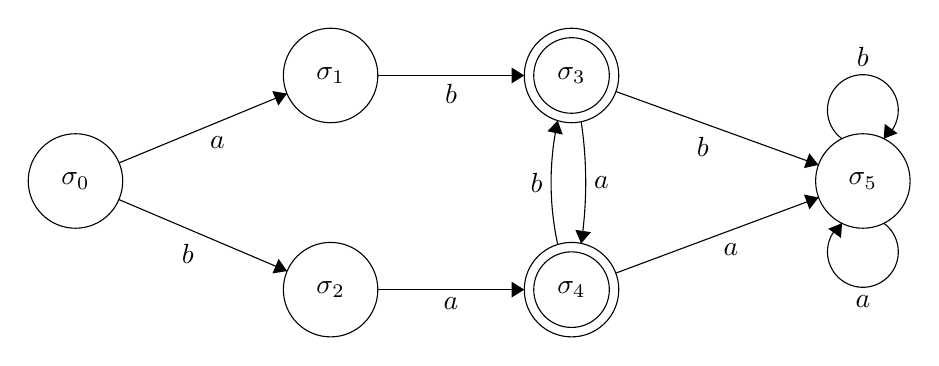
\begin{tikzpicture}[scale=0.2]
		\tikzstyle{every node}+=[inner sep=0pt]
		\draw [black] (11.4,-26) circle (3);
		\draw (11.4,-26) node {$\sigma_0$};
		\draw [black] (27.6,-19.3) circle (3);
		\draw (27.6,-19.3) node {$\sigma_1$};
		\draw [black] (27.6,-32.9) circle (3);
		\draw (27.6,-32.9) node {$\sigma_2$};
		\draw [black] (42.9,-19.3) circle (3);
		\draw (42.9,-19.3) node {$\sigma_3$};
		\draw [black] (42.9,-19.3) circle (2.4);
		\draw [black] (42.9,-32.9) circle (3);
		\draw (42.9,-32.9) node {$\sigma_4$};
		\draw [black] (42.9,-32.9) circle (2.4);
		\draw [black] (61.4,-26) circle (3);
		\draw (61.4,-26) node {$\sigma_5$};
		\draw [black] (14.17,-24.85) -- (24.83,-20.45);
		\fill [black] (24.83,-20.45) -- (23.9,-20.29) -- (24.28,-21.21);
		\draw (20.41,-23.16) node [below] {$a$};
		\draw [black] (14.16,-27.18) -- (24.84,-31.72);
		\fill [black] (24.84,-31.72) -- (24.3,-30.95) -- (23.91,-31.87);
		\draw (18.53,-29.96) node [below] {$b$};
		\draw [black] (30.6,-19.3) -- (39.9,-19.3);
		\fill [black] (39.9,-19.3) -- (39.1,-18.8) -- (39.1,-19.8);
		\draw (35.25,-19.8) node [below] {$b$};
		\draw [black] (30.6,-32.9) -- (39.9,-32.9);
		\fill [black] (39.9,-32.9) -- (39.1,-32.4) -- (39.1,-33.4);
		\draw (35.25,-33.4) node [below] {$a$};
		\draw [black] (42.025,-30.034) arc (-167.67645:-192.32355:18.432);
		\fill [black] (42.02,-22.17) -- (41.37,-22.84) -- (42.34,-23.05);
		\draw (41.1,-26.1) node [left] {$b$};
		\draw [black] (43.513,-22.235) arc (8.51362:-8.51362:26.108);
		\fill [black] (43.51,-29.97) -- (44.13,-29.25) -- (43.14,-29.1);
		\draw (44.3,-26.1) node [right] {$a$};
		\draw [black] (45.72,-20.32) -- (58.58,-24.98);
		\fill [black] (58.58,-24.98) -- (58,-24.24) -- (57.66,-25.18);
		\draw (51.23,-23.18) node [below] {$b$};
		\draw [black] (45.71,-31.85) -- (58.59,-27.05);
		\fill [black] (58.59,-27.05) -- (57.66,-26.86) -- (58.01,-27.8);
		\draw (53.03,-29.97) node [below] {$a$};
		\draw [black] (60.077,-23.32) arc (234:-54:2.25);
		\draw (61.4,-18.75) node [above] {$b$};
		\fill [black] (62.72,-23.32) -- (63.6,-22.97) -- (62.79,-22.38);
		\draw [black] (62.723,-28.68) arc (54:-234:2.25);
		\draw (61.4,-33.25) node [below] {$a$};
		\fill [black] (60.08,-28.68) -- (59.2,-29.03) -- (60.01,-29.62);
	\end{tikzpicture}
\end{center}

\subsubsection*{37.}
Yikes.
\end{document}
